\documentclass[fleqn]{article}
%\textwidth=6in
%\textheight=9in
%\pagestyle{empty}
\usepackage{amsmath,amssymb,amsthm,ragged2e,siunitx,graphicx,multicol,wrapfig,mathtools,parskip}
\usepackage[margin=0.7in]{geometry}
\usepackage[T1]{fontenc}
\usepackage[utf8]{inputenc}
\usepackage[dvipsnames]{xcolor}
\usepackage[export]{adjustbox}
\newtheorem{thm}{{\sc Theorem}}[section]
\newtheorem{prop}[thm]{{\sc Proposition}}
\newtheorem{cor}[thm]{{\sc Corollary}}
\newtheorem{lem}[thm]{{\sc Lemma}}
\newtheorem{df}[thm]{{\sc Definition}}

\DeclarePairedDelimiter\ceil{\lceil}{\rceil}
\DeclarePairedDelimiter\floor{\lfloor}{\rfloor}

\DeclareMathOperator{\sech}{sech}
\DeclareMathOperator{\csch}{csch}

% automatically makes new paragraphs have no indent
\setlength{\parindent}{0pt}

% new command for underscore
\newcommand{\underscore}{\underline{\hspace{1cm}}}

% this is a command for the space between asterisk or plus and the problem statement
\newcommand{\gap}{\hspace{.25cm}}

\newcommand*\colvec[1]{\begin{bmatrix*}[r]#1\end{bmatrix*}} 

% Uncomment this to write vectors bolded 
\renewcommand{\vec}[1]{\boldsymbol{#1}}

% Uncomment this to write vectors bolded AND with arrow on top
\newcommand{\avec}[1]{\overrightarrow{\boldsymbol{#1}}}
% this notation has an arrow on top of vector which is redundant if it is bolded

% Uncomment this to write vectors unbolded with long arrow on top
% \renewcommand{\vec}[1]{\overrightarrow{#1}}

% this is a command for a coefficient matrix with right-aligned entries (good for aligning negative signs)
\newcommand{\mat}[1]{\begin{bmatrix*}[r]#1\end{bmatrix*}} 

% this is a command for a coefficient matrix with center-aligned entries (good for aligning negative signs)
\newcommand{\cmat}[1]{\begin{bmatrix*}[c]#1\end{bmatrix*}} 

% this is a command for a DETERMNINANT matrix with right-aligned entries (good for aligning negative signs) (ABSOLUTE VALUE BARS)
\newcommand{\vmat}[1]{\begin{vmatrix*}[r]#1\end{vmatrix*}} 

% this is a command for black squares (useful for pivots in matrices) when already in math mode (between $ signs)
\newcommand{\bsq}{\blacksquare}






%%  environment for AUGMENTED  matrices
\newenvironment{amatrix}[1]{%
  \left[\begin{array}{@{}*{#1}{r}|r@{}}
}{%
  \end{array}\right]
}


%%% new command for Augmented BAR alone (helpful for putting augmented bar somewhere in middle of matrix)
\newcommand\aug{\fboxsep=-\fboxrule\!\!\!\fbox{\strut}\!\!\!}

% define new color (i.e. pink)
\definecolor{mypink1}{rgb}{0.858, 0.188, 0.478}

% define new color (i.e. medium green)
\definecolor{MediumGreen}{rgb}{0.1, 0.8, 0.65}

% define new color (i.e. dark purple)
\definecolor{DarkPurple}{rgb}{0.6, 0, 0.6}

% this is a command for the size of headers
\newcommand{\header}[1]{\noindent{\Large \textcolor{mypink1}{\textbf{#1}}}}

% this is a command for the size of subheaders
\newcommand{\subheader}[1]{\noindent{\large \textcolor{red}{\textbf{#1}}}}

% this is a command for answers in RED on same line with a space between problem and answer
\newcommand{\sred}[1]{\hspace{1cm} \textcolor{red}{#1}}

% this is a command for answers in RED on same line with NO space between problem and answer
\newcommand{\red}[1]{\textcolor{red}{#1}}

% this is a command for answers in PURPLE on same line with NO space between problem and answer
\newcommand{\DarkPurple}[1]{\textcolor{DarkPurple}{#1}}

% this is a command for answers in GREEN on same line with NO space between problem and answer
\newcommand{\MediumGreen}[1]{\textcolor{MediumGreen}{#1}}

% this is a command for answers in BLUE on same line with a space between problem and answer
\newcommand{\sblue}[1]{\hspace{1cm} \textcolor{blue}{#1}}

% this is a command for answers in BLUE on same line with NO space between problem and answer
\newcommand{\blue}[1]{\textcolor{blue}{#1}}


% this is a command for defining EXAMPLES
\theoremstyle{definition}
\newtheorem{exmp}{Example}[section]




\begin{document}

\centerline{\Large \bf Math Seminar Template Notes}
\centerline{\large \bf Day 2 (Sums and Proof by Induction)}
\vspace{\baselineskip}

%\noindent \underline{\hspace{18cm}}

\header{Day 2 (Sums and Proof by Induction) } \\


\noindent\fbox{%
\parbox{\textwidth}{
\subheader{Overview} \\ 
%\vspace{0.25cm}
\textbf{\underline{Goals}} 
\begin{enumerate}
\item Compute infinite sums 
\item Prove statements using a proof by induction 
\end{enumerate}
\vspace{.25cm}
}}

\vspace{0.2cm}


\subheader{Zeno's Paradox} 

\textbf{Ex 1:} Achilles is having a race with a tortoise, but Achilles is faster than the tortoise so he gives the tortoise a head start. 
    \begin{itemize}
    \item \textbf{Step 1:} The race starts! In some amount of time, Achilles reaches the point where the tortoise started. By that time, the tortoise has moved forward a little. 
    \item \textbf{Step 2:} In some additional amount of time, Achilles reaches the point where the tortoise got to in Step 1. By that time, the tortoise has moved forward a little again. 
    \item \textbf{Step 3:} In some additional amount of time, Achilles reaches the point where the tortoise got to in Step 2. By that time, the tortoise has moved forward a little again. 
    \item This process continues on forever. Each time Achilles reaches the point where the tortoise previously was, the tortoise has moved forward a little (it's a smaller distance at each step, but a positive distance)
    \end{itemize}

\vspace{.25cm}
\textbf{Discussion Question:} Since the process described above continues indefinitely, how can Achilles ever catch the tortoise? 

%image aligned
%%
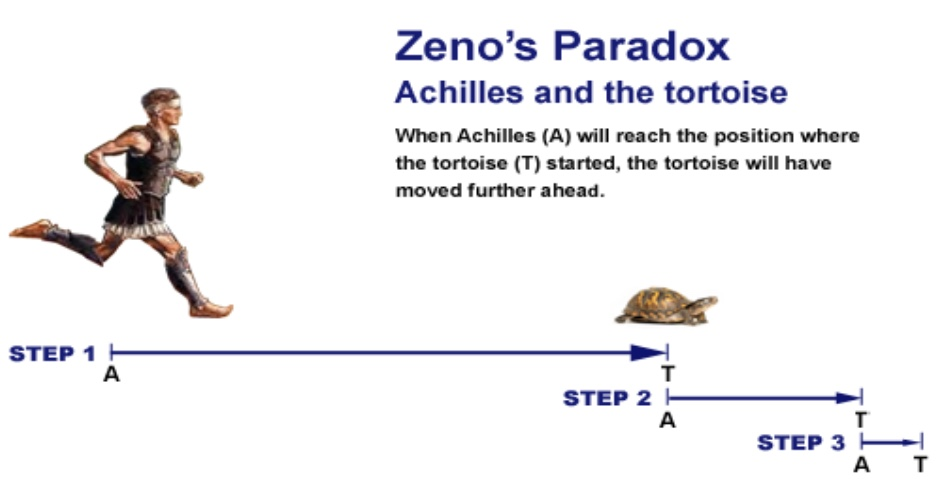
\includegraphics[scale=0.4, center]{Zeno.jpeg}
\vspace{-10pt}

\vspace{1cm}
\textbf{Follow up:} Suppose I need to walk 1 mile, but I decide to break it up in the following way. First, I walk half this distance (so 1/2 mi). Then, I walk half of the remaining distance (so 1/4 mi). Then, I walk half of the remaining distance (so 1/8 mi). I continue on in this way ``forever," perpetually going half of the remaining distance. 

\vspace{.25cm}
\textbf{Q:} How far do I end up walking?



%%%
\newpage

\subheader{Geometric Series}

%\subheader{What is $\displaystyle{ \frac{1}{2} + \frac{1}{4} + \frac{1}{8} + \ldots }$?}

%%%% something in a box
\noindent\fbox{%
\parbox{\textwidth}{\vspace{.25cm}
\textbf{Def:} When we add a bunch of terms together, we sometimes call this a \textbf{series}. 

    \vspace{.5cm}
    \hspace{1cm} (a) $\displaystyle{ \frac{1}{2} + \frac{1}{4} + \frac{1}{8} + \ldots }$ is an infinite series

    \vspace{.25cm}
    \hspace{1cm} (b) $4+12+36+108 + \ldots + 4(3)^{10}$ is a finite series

    \vspace{.25cm}
    \hspace{1cm} (c) $\displaystyle{ 1 + \frac{1}{2} + \frac{1}{3} + \frac{1}{4} + \ldots }$ is an infinite series

\vspace{.5cm}
\textbf{Def:} When we can get from one term to the next term of a series by multiplying by the same constant factor, all the way through the series, we call it a \textbf{geometric series}. A finite geometric series has the form:

    \vspace{.25cm}
    \hspace{1cm} $a + ar + ar^2 + ar^3 + \ldots ar^n$
\vspace{.25cm}   
}}
%%% end box

\vspace{.25cm}
Let's prove a formula for the sum of a geometric series. We call the first term, $a$, and the common ratio, $r$.

\vspace{.25cm}
    \hspace{1cm} Let \hspace{.35cm} $S = a + ar + ar^2 + ar^3 + \ldots ar^n$

\vspace{.25cm}
    \hspace{1cm} Then \hspace{0cm} $Sr = \hspace{.5cm} $

\vspace{3cm}
\textbf{Q:} What does this become when we have infinitely many terms (i.e. $n \rightarrow \infty$)? 

    \vspace{.25cm}
    \hspace{1cm} $S = \displaystyle{ \frac{ \hspace{1.5cm}}{ } }$ \hspace{.5cm} as long as $\underline{\hspace{1cm}} \leq r \underline{\hspace{1cm}}$

\vspace{1cm}



\textbf{Ex 2:} Let's compute $0.999 \ldots$ in a few different ways. 

\vspace{.25cm}
\textbf{Method 1}

\vspace{.1cm}
(a) Can you write this number as an infinite geometric series? I'll get you started. Let me call this number $S$: 

    \hspace{1cm} $S = \displaystyle{ \frac{9}{10} + }$

\vspace{.5cm}
(b) Identify what the first term $a$ and the common ratio $r$ are. 

\vspace{1.5cm}
(c) Plug these into the formula for the sum of an infinite geometric series. 


%%%
\newpage

\textbf{Method 2}

\vspace{1.25cm}
Let $S = 0.999 \ldots$

\vspace{2.5cm}
Try multiplying both sides by something ``nice." Think back to the trick we used to prove the sum of a geometric series and what we multiplied both sides by there. 

\vspace{.25cm}
This will now give you a 2nd equation. Keep going like we did in the proof of the sum of a geometric series until you solve for $S$.  

\vspace{1cm}

\subheader{What is Induction?} 

Suppose we are trying to show some statement, $P(n)$, is true for all integers $n \geq 1$. 

\vspace{.05cm}
	\hspace{1cm} $\displaystyle{ \Bigg( }$ e.g. $P(n)$ might be the statement $\displaystyle{1^2+2^2+3^2 + \ldots + n^2 = \frac{n(n+1)(2n+1)}{6} }$ $\displaystyle{ \Bigg) }$

\vspace{.25cm}
It's hard to show such statements using our earlier methods for series.

\vspace{.25cm}
%%%% something in a box
\noindent\fbox{%
\parbox{\textwidth}{\vspace{.25cm}
\textbf{Idea:} Represent, $P(1), P(2), P(3), \ldots $ using \textbf{dominoes}.  

%image centered
%%
\begin{center}
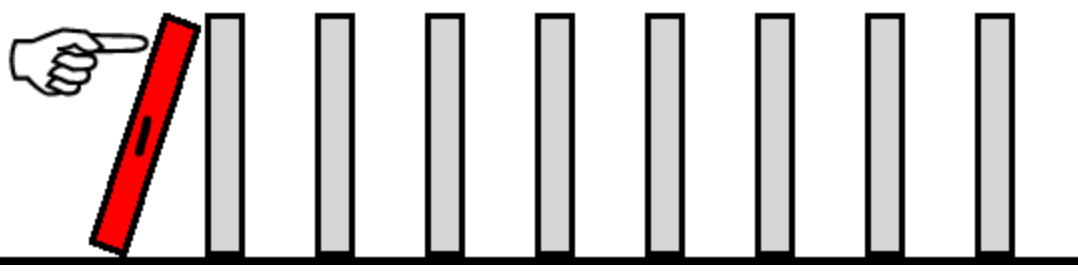
\includegraphics[scale=0.5]{InductionDominoes}
\end{center} 
% \vspace{-20pt}

Suppose we know the following: 

	\vspace{.2cm}
	\begin{enumerate}
	\item Domino \underline{\hspace{1cm}} falls

	\vspace{.25cm}
	\item If domino $k$ falls, then domino \underline{\hspace{1.5cm}} also falls (for any positive integer $k$)
	\end{enumerate}

\vspace{.25cm}
\textbf{Outcome:} Then, \underline{\hspace{2cm}} dominoes will fall!
\vspace{.25cm}   
}}
%%% end box



\vspace{.25cm}
%%%% something in a box
\noindent\fbox{%
\parbox{\textwidth}{\vspace{.25cm}
\hspace{5cm} \textbf{Principle of Mathematical Induction} 

\vspace{.25cm}
To prove a statement, $P(n)$, is true for all integers $n \geq 1$ ($n \in \mathbb{Z}^+$), using \textbf{induction}, there are 2 steps:

	\vspace{.25cm}
	\begin{enumerate}
	\item \textbf{(Base Step):} Show \underline{\hspace{1cm}} is true

	\vspace{.25cm}
	\item \textbf{(Inductive Step):} Assume \underline{\hspace{1.5cm}} is true for an arbitrary $k \in \mathbb{Z}^+$, and show this implies that \underline{\hspace{1.75cm}} is true. 

%	\vspace{.25cm}
%	\hspace{1cm} i.e. show $\underline{\hspace{1.5cm}} \rightarrow \underline{\hspace{1.75cm}}$
	\end{enumerate}
\vspace{.25cm}   
}}
%%% end box


%%%
\newpage

\subheader{Induction Proof: Summation}

\textbf{Ex 3:} Prove that for all positive integers $n$, 
	$$\sum_{i=1}^{n} i^2 = \hspace{5cm} = \frac{n(n+1)(2n+1)}{6} $$

\textbf{Pf:} Let's proceed by \underline{\hspace{6cm}}. 

\vspace{.25cm}
\MediumGreen{Step 0: Identify $P(n)$}

\vspace{.25cm}
	\hspace{1cm} $P(n):$ 

\vspace{1cm}

\MediumGreen{Step 1: Prove the base step} \hspace{1cm} (usually \underline{\hspace{2cm}} but depends on problem statement) 

	\vspace{.25cm}
	\hspace{1cm} Is \underline{\hspace{1.5cm}} true?


\vspace{2cm} 
\MediumGreen{Step 2: Prove the inductive step } \hspace{.5cm} % (show $P(k) \rightarrow P(k+1)$)


\vspace{.5cm}

Let $k \in \underline{\hspace{1cm}}$. Assume \underline{\hspace{1.5cm}} is true, namely that 

\vspace{8cm} 
By induction, \hspace{7cm} for all $n \in \underline{\hspace{1cm}}$. 



\vspace{.25cm}
%%%% something in a box
\noindent\fbox{%
\parbox{\textwidth}{\vspace{.25cm}
\textbf{Induction \MediumGreen{Pros}/\red{Cons}}

\vspace{.5cm}
	\begin{enumerate}
	\item \MediumGreen{(Pro):} It's helpful for proving many statements of the form ``prove $P(n)$ for all integers $n \geq \ldots$" 

	\vspace{.25cm}
	\item \red{(Con):} It doesn't give insights about why the result is true conceptually
	\end{enumerate}
\vspace{.25cm}   
}}
%%% end box


%%%
\newpage

\subheader{Practice Problems}

\vspace{.25cm}
%%%% something in a box
\noindent\fbox{%
\parbox{\textwidth}{\vspace{.25cm}
\hspace{5cm} \textbf{Principle of Mathematical Induction} 

\vspace{.25cm}
To prove a statement, $P(n)$, is true for all integers $n \geq 1$ ($n \in \mathbb{Z}^+$), using \textbf{induction}, there are 2 steps:

	\vspace{.25cm}
	\begin{enumerate}
	\item \textbf{(Base Step):} Show $P(1)$ is true

	\vspace{.25cm}
	\item \textbf{(Inductive Step):} Assume \underline{\hspace{1.5cm}} is true for an arbitrary $k \in \mathbb{Z}^+$, and show this implies that \underline{\hspace{1.75cm}} is true. 

%	\vspace{.25cm}
%	\hspace{1cm} i.e. show $\underline{\hspace{1.5cm}} \rightarrow \underline{\hspace{1.75cm}}$
	\end{enumerate}
\vspace{.25cm}   
}}
%%% end box

\vspace{.25cm}


\begin{enumerate}

\item In our last class, we saw that $\displaystyle{1+2+3+ \ldots + n = \frac{n(n+1)}{2}}$ where $n$ is a positive integer. Now let's prove this using induction. 

%%%
\newpage

\item Prove that $\displaystyle{1^3 + 2^3 + 3^3 + \ldots + n^3 = \left( \frac{n(n+1)}{2} \right)^2}$ using induction.

%%%
\newpage 

\item Prove that $4^n-1$ is divisible by $3$ for all positive integers $n$ using induction. 

\vspace{.25cm}
\textbf{Hint:} One way to say an integer, $x$ is divisible by 3 with an equation is to say that $x=3j$ where $j$ is some integer. 


%%%
\newpage

\item The \textbf{Fibonacci numbers} are defined to be $f_1=0, f_2=1$, and $f_{n} = f_{n-1} + f_{n-2}$ for integers $n \geq 2$. 

\vspace{.25cm}
(a) Write out the first 7 Fibonacci numbers. 

\vspace{1.5cm}
(b) Prove that $f_1 + f_2 + f_3 + \ldots + f_n = f_{n+2} - 1$ using induction. 



\end{enumerate}




\end{document}





%%%% something in a box
\noindent\fbox{%
\parbox{\textwidth}{\vspace{.25cm}
\textbf{Strategies to Show Inductive Step}

\vspace{.25cm}
	\begin{enumerate}
	\item Start with $P(k)$ and do stuff to \underline{\hspace{4cm}} so it becomes $P(k+1)$

	\vspace{.25cm}
	\item Start with one side/part of $P(k+1)$ and use the assumption that \underline{\hspace{4cm}} to get the rest of $P(k+1)$
	\end{enumerate}
\vspace{.25cm}   
}}
%%% end box




\begin{multicols}{5} 
Type 
\columnbreak 

Symbol 
\columnbreak

Definition 
\columnbreak

\hspace{1cm}
 \columnbreak
 
\hspace{1cm}
\end{multicols}






%%%%%%%%%%%%%%%%%%%%%%%%%%%%%%%%%%%%%%%%%%%%%%%%%%%%%%%%%




%image aligned
%%
\includegraphics[scale=0.7, right]{BlankAxes}
\vspace{-10pt}


%image centered
%%
\begin{center}
\includegraphics[scale=1.4]{SinCosTanDrawGraphs}
\end{center} 
\vspace{-20pt}



%%% incorrect/correct show something with 2 approaches
\vspace{.25cm} 
\begin{multicols}{2} 
\red{\underline{Incorrect}} \columnbreak

\MediumGreen{\underline{Correct}} 
\end{multicols}


%%% Scratch work for proof
\hspace{7cm} \MediumGreen{\underline{Scratch Work}}
\begin{multicols}{2} 
\hspace{4cm} \MediumGreen{\underline{Given/Know}} \columnbreak

\MediumGreen{\underline{Want to show}} 
\end{multicols}

\vspace{2.5cm} 



%%%% something in a box
\noindent\fbox{%
\parbox{\textwidth}{\vspace{.25cm}
\textbf{Def:} \\ (1) The \DarkPurple{intersection} of sets $A$ and $B$ is the set of all elements in \textbf{both} $A$ \textbf{and} $B$, denoted $\underline{\hspace{2cm}}$. 
\vspace{.25cm}   
}}
%%% end box


%%% big row reduction arrow
\xrightarrow{\hspace*{2cm}}  



%%% table with extra vertical spacing
\begin{tabular}{ c|c|c } 
$f'(x)$ &  $f(x)$  &  $F(x)$  \\ \hline
\rule{0pt}{3ex}           &  $x^n$  &             \\
 \rule{0pt}{5ex}          &  $\displaystyle{x^{-1}=\frac{1}{x}}$   &             \\
\rule{0pt}{5ex}           &  $e^x$  &             \\
\rule{0pt}{5ex}           &  $e^{kx}$  &             \\
\rule{0pt}{5ex}           &  $g(x) \pm h(x)$  &             \\
\rule{0pt}{5ex}           &  $cg(x)$  &             \\
\rule{0pt}{5ex}           &  $g(x)h(x)$  &             \\
\rule{0pt}{5ex}           &  $\displaystyle{\frac{g(x)}{h(x)}}$  &             \\
\end{tabular}



%%% coefficient matrix template
$A = \mat{ 1 & 0 & 1 & 2 & 2 \\ 0 & 0 & 1 & 0 & 1 \\ 2 & 0 & 1 & 4 & 3 }$


%%% augmented matrix template (the number in brackets indicates which column the augmented bar will be placed AFTER)
$\begin{amatrix}{5}
1 & -1 & 0 & -5 & 0 & -9  \\ 
0 & 0  & 1 &  4 & 0 & 4 \\ 
0 & 0  & 0 &  0 & 1 & 3  
 \end{amatrix}$
 
 
 
 %%%% template for multiple alignment points in system of equations
 $\begin{alignedat}{3}
		x_1 &+ x_2 &&- x_3 &&= -6 \\
		3x_1 &+ x_2 &&+x_3  &&= 8 \\
		4x_1 &+ 2x_2 &&      &&= 2 \\
		\end{alignedat}$
